\section{Macroeconomic Forecasting Application}
\label{sec:forecasting_application}
To validate the model behavior in a real-world scenario \textcite{hauzenberger_combining_2021} conduct an empirical forecasting application on a popular macroeconomic dataset, namely the \textcite{mccracken_fred-md_2015} dataset.

This dataset spans $m = 165$ macroeconomic and financial variables in quarterly resolution from 1959:Q1 up until 2018:Q4. The target variables of the forecasting exercise are the traditional ones: Output (GDPC1), consumer price inflation (CPIAUCSL), and the Federal Funds Rate (FEDFUNDS).

\subsection{Forecasting Exercise Setup}
\label{subsec:forecasting_setup}
To evaluate the performance of sparse BVAR models, the authors compare different sparse models with different hyperparameters to other competitive models specified below.

They rely on a recursive forecasting design and compute $h \in \{1,4,8\}$-step-ahead forecasts. Recursive means that the training set, which spans the initial observations from 1959:Q1 to 1989:Q4 (first 30 years), is expanded one step at a time to recursively compute out-of-sample forecasts for the next $h$ time steps.

The metrics used to evaluate the model performance on the hold-out set are the root-mean-squared-forecast-error (RMSE) for point-estimates and log predictive likelihoods (LPLs) for predictive densities (see Appendix \ref{app:rmse} and \ref{app:lpl}).

In order to give meaning to these metrics \textcite{hauzenberger_combining_2021} compare different models with different hyperparameter setups against each other. Ideally, sparsification should select the most important variables automatically which is why the \textbf{L-VAR} model features all $m = 165$ variables of the dataset. This goes in line with existing literature highlighting that it is important to exploit larger information sets \parencite{banbura_large_2010,giannone_prior_2015,koop_forecasting_2013}. This model size is then compared to other model sizes:

\paragraph{S-VAR} This model is considered the baseline model and all metrics are computed relative to the metrics of this model. It is a simple BVAR model featuring only the three target variables.

\paragraph{M-VAR} The total number of variables included in this model are $m = 21$ variables. This extends the \textbf{S-VAR} by 18 financial market variables.

\paragraph{FA-VAR} This factor-augmented (FA) model attempts to exploit the full information set by extending the \textbf{S-VAR} with three principal components extracted from all other variables except the three target variables.
\\\phantomsection\par %\phantomsection fills out the line internally for LaTeX to avoid "underfull hbox" notifications
All models feature $p = 5$ lags and are estimated with the Minnesota prior setup presented in Section~\ref{subsec:prior_setup}. In addition, a non-conjugate BVAR model with the SSVS prior is considered \parencite{george_bayesian_2008}. However, this model is not computed for the \textbf{L-VAR} model size due to the additional computational burden of the non-conjugate prior (meaning that the posterior needs to be simulated).

The choice of hyperparameters differs for the \textbf{L-VAR} in comparison to the other model sizes. For all models except for the \textbf{L-VAR} the $\theta_1$ hyperparameter of the Minnesota prior (which is part of the $\delta$ hyperparameter tuple specified in Section~\ref{subsec:prior_setup}) is determined by maximizing the marginal likelihood over a grid of search values. This procedure is unfeasible for the \textbf{L-VAR} which is why results are reported for $\theta_1 \in \{0.025,0.05,0.075\}$. Large $\theta_1$ values put less weight on shrinkage while small values put more weight on shrinkage. As a consequence, the SAVS estimator used to ex-post sparsify estimates leads to a more sparse model if $\theta_1$ is small. The values of $\lambda$ (see Section~\ref{subsubsec:sparsification_alpha}) and $w$ (see Section~\ref{subsubsec:sparsification_sigma}) are also reported over a grid for $\lambda \in \{0.01,0.1,0.5,1\}$ and $w = \frac{\lambda}{10}$.

\subsection{Average Point- and Density Forecast Performance}
\label{subsec:avg_forecast_performance}
The average point- and density forecast performances as evaluated by the RMSE and the LPLs in comparison to the baseline \textbf{S-VAR} only reveal mixed evidence in favor of larger sparse models. The average forecast performance is the out-of-sample model performance averaged over the complete hold-out set (1990:Q1 to 2018:Q4). It is reported separately for each forecasting horizon $h \in \{1,4,8\}$ and the grid of hyperparameters specified in Section~\ref{subsec:forecasting_setup}. In the following, the results are summarized and the detailed results can be found in \textcite[Tables 2, 3, 4, and 5]{hauzenberger_combining_2021}.

Generally, one can observe that multi-step-ahead forecasts for $h \in \{ 4 , 8 \}$ benefit from larger information sets. \textbf{L-VAR} and \textbf{M-VAR} models perform better on average for these forecasts. Regarding sparse versus non-sparse models, one can observe that using ex-post sparsification and the Minnesota prior works well, especially for longer run forecasts of output and interest rate. Sparse models using the non-conjugate SSVS prior never dominate for point-estimates and only in rare cases for density forecasts. The main driver of bad performance of both sparse and large models is revealed by the marginal LPL of inflation \parencite[p.~319, Table~4]{hauzenberger_combining_2021}. The \textbf{S-VAR} and \textbf{FA-VAR} perform best while the density forecasting performance of \textbf{L-VAR} models and especially sparse \textbf{L-VAR} models drops sharply. This is a well-known result in central bank practice \parencite{giannone_prior_2015} and investigated further in Section~\ref{subsec:forecasting_over_time}. For output and interest rate, this behavior is reversed meaning that larger and more sparse models perform better overall.

Finally, it is important to note that sparsification only very rarely hurts forecasting performance in a significant manner which the authors validate by computing Model Confidence Sets (MCS) on a 25\% significance level. For point-forecasting performance, the MCS contain between 26 and 33 out of 33 models in total with large shares of models using SAVS across all target variables. In terms of density forecasting performance, the MCS are smaller for output and interest rate with larger shares of models using SAVS. For inflation, the MCS is larger again and favors smaller models as discussed previously.

\subsection{Density Forecast Performance over time}
\label{subsec:forecasting_over_time}
To investigate further how large and sparse models using SAVS perform, it is interesting to consider the forecasting performance over time. Discriminating between different time periods allows identifying reasons for performance drops.

Figure \ref{fig:lpl_one_year_ahead} depicts the cumulative sum of log predictive likelihoods for one-year-ahead ($h = 4$) forecasts over time for the complete hold-out period. The left-hand side is the period before the financial crisis while the right-hand side illustrates the period during and after the financial crisis.
\begin{figure}
    \centering
    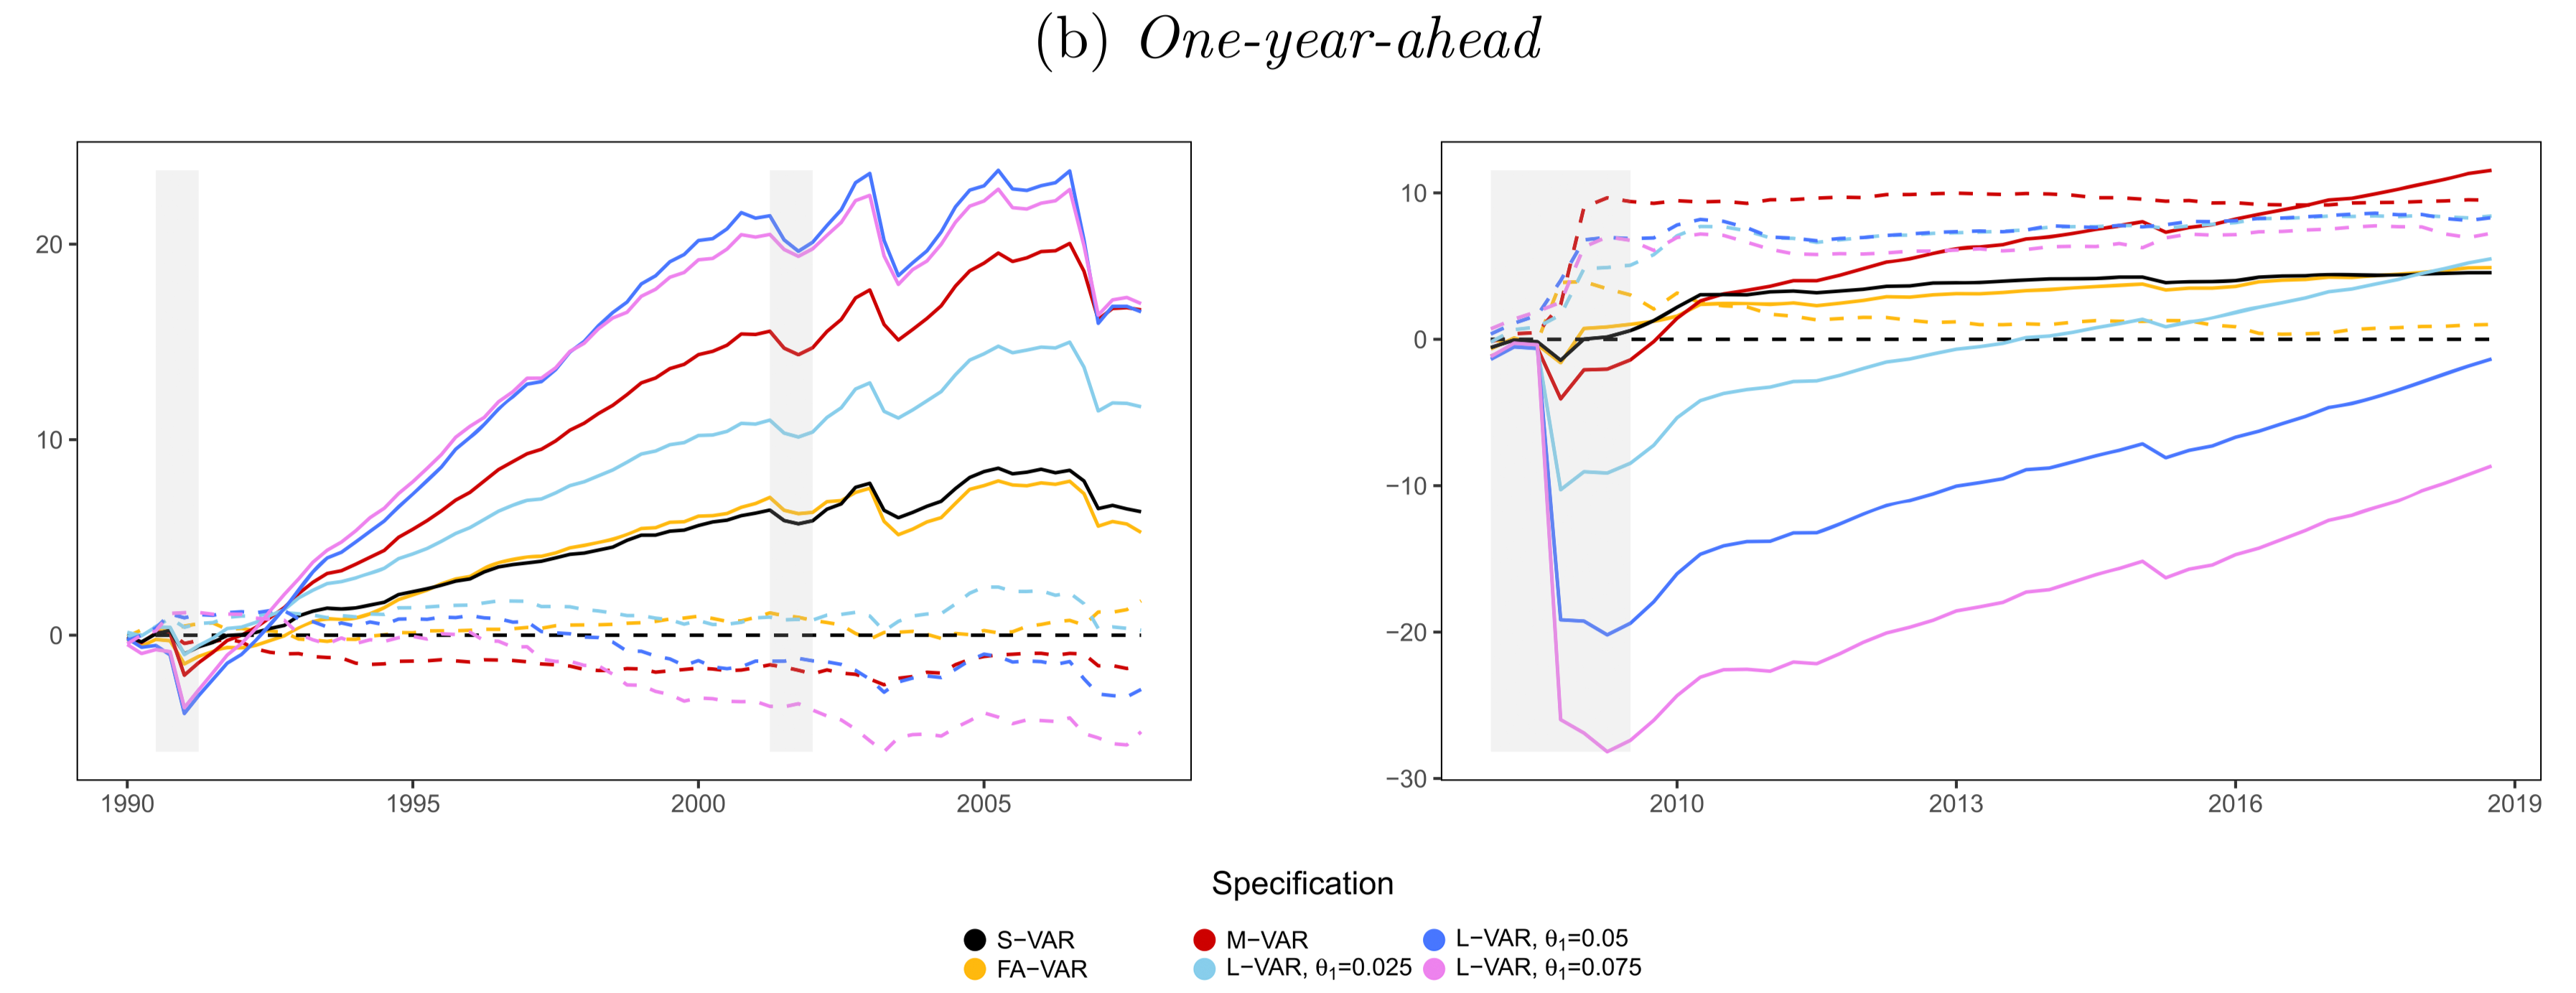
\includegraphics[width=\textwidth]{figures/lpl_one_year_ahead.png}
    \caption{Cumulative sum of LPLs for one-year-ahead forecasts before (left), during, and after (right) the financial crisis \parencite[Figure~2]{hauzenberger_combining_2021}. Solid lines indicate models with SAVS while dashed lines represent the non-sparse counterpart without SAVS. Large values for $\theta_1$ put less weight on shrinkage leading to a more dense model after SAVS. Higher values are better.}
    \label{fig:lpl_one_year_ahead}
\end{figure}
One can observe that, before the financial crisis (left plot), large models using SAVS and the \textbf{M-VAR} using SAVS perform very well. Especially the large models with moderate shrinkage and SAVS (solid blue and magenta lines) are superior to all other models. This means that there is strong evidence in favor of large and sparse models before the financial crisis. 

On the other hand side, this pattern is reversed during the financial crisis as depicted by the gray shaded background in the right plot. All \textbf{L-VARs} with SAVS exhibit by far the strongest drop in density forecasting performance. This reflects the previously observed fact in Section~\ref{subsec:avg_forecast_performance} that inflation forecasts are the main driver of bad performance. The heavy misestimation of inflation seems to impact the joint forecasting performance of the sparse \textbf{L-VAR} models dramatically. During the time of the financial crisis, models without SAVS and the \textbf{M-VAR} and \textbf{FA-VAR} with SAVS are more stable. Nonetheless, after the financial crisis, the larger models, such as all \textbf{L-VARs} and the \textbf{M-VAR} with SAVS, return to the good performance like before the crisis which can be seen by the steep increase of the curve after the end of the crisis. Similar results can be observed for one-quarter-ahead forecasts \parencite[Figure~2]{hauzenberger_combining_2021}.

A reason for the decline in forecasting performance during the financial crisis is most likely related to the bias-variance trade-off introduced in Section~\ref{subsec:shrinkage_and_sparsity}. A researcher typically applies shrinkage and sparsity techniques to a model to reduce the predictive variance while sacrificing bias. If the hyperparameters are chosen carefully this usually comes with the benefit of better generalization to new data. However, as one can see by the decline of performance during the financial crisis, a reduced predictive variance also means that the model is less likely to capture outliers in the data -- like the financial crisis. This instance highlights the bias-variance trade-off very well: Sacrificing bias for a smaller predictive variance leads to great forecasting performance during ``normal'' times but comes with the drawback of a decline in performance during ``unusual'' times like the financial crisis.
